

%+++++++++++++++++++++++++++++++++++++++++++
\section{Temporal Difference Learning}
%-------------------------------------------

待重读的资源:
\begin{itemize}
%\setlength{\itemsep}{0pt}
%\setlength{\parsep}{0pt}
\setlength{\parskip}{0pt}
\item[-]
\url{https://trunghng.github.io/artificial-intelligent/reinforcement-learning/2022/04/08/td-learning.html}

\item[-]
\url{https://web.stanford.edu/class/cme241/lecture_slides/rich_sutton_slides/11-12-TD.pdf}
\end{itemize}

\cite{ODSC2020}

The temporal difference learning algorithm was introduced by Richard S. 
Sutton in 1988.  The reason the temporal difference learning method became 
popular was that it combined the advantages of dynamic programming and the 
Monte Carlo method. But what are those advantages? 

This section is an excerpt from the book  Deep Reinforcement Learning with 
Python, Second Edition  by  Sudharsan Ravichandiran – a comprehensive guide 
for beginners to become proficient in implementing state-of-the-art RL and 
deep RL algorithms.  

%+++++++++++++++++++++++++++++++++++++++++++
\subsection{the advantages and disadvantages of DP and the MC method}

Dynamic programming — the advantage of the DP method is that it uses the 
Bellman equation to compute the value of a state. That is, we have learned 
that according to the Bellman equation, the value of a state can be obtained 
as the sum of the immediate reward and the discounted value of the next 
state. This is called bootstrapping. That is, to compute the value of a 
state, we don't have to wait till the end of the episode, instead, using 
the Bellman equation, we can estimate the value of a state just based on 
the value of the next state, and this is called bootstrapping.  

Remember how we estimated the value function in DP methods (value and policy 
iteration)? We estimated the value function (the value of a state) as:
$$
V(s) = \sum_{s'}P_{ss'}^a\left[ R_{ss'}^a + \gamma V(s') \right]
$$

As you may recollect, we learned that in order to find the value of a state, 
we didn't have to wait till the end of the episode. Instead, we bootstrap, 
that is, we estimate the value of the current state $V(s)$ by estimating the 
value of the next state $V(s')$. 

However, the disadvantage of DP is that we can apply the DP method only when 
we know the model dynamics of the environment. That is, DP is a model-based 
method and we should know the transition probability in order to use it. 
When we don't know the model dynamics of the environment, we cannot apply 
the DP method.  

Monte Carlo method — The advantage of the MC method is that it is a 
modelfree method, which means that it does not require the model dynamics 
of the environment to be known in order to estimate the value and $Q$ 
functions.  

However, the disadvantage of the MC method is that in order to estimate the 
state value or $Q$ value we need to wait until the end of the episode, and 
if the episode is long then it will cost us a lot of time. Also, we cannot 
apply MC methods to continuous tasks (non-episodic tasks).  

Now, let's get back to temporal difference learning. The TD learning 
algorithm takes the benefits of the DP and the MC methods into account. So, 
just like in DP, we perform bootstrapping so that we don't have to wait 
until the end of an episode to compute the state value or $Q$ value, and 
just like the MC method, it is a model-free method and so it does not 
require the model dynamics of the environment to compute the state value 
or $Q$ value. Now that we have the basic idea behind the TD learning 
algorithm, let's get into the details and learn exactly how it works. 

We can use the TD learning algorithm for both the prediction and control 
tasks, and so we can categorize TD learning into:  
\begin{itemize}
\item
TD prediction

\item
TD control
\end{itemize}

In the prediction method, a policy is given as an input and we try to 
predict the value function or Q function using the given policy. If we 
predict the value function using the given policy, then we can say how good 
it is for the agent to be in each state if it uses the given policy. That 
is, we can say what the expected return an agent can get in each state if 
it acts according to the given policy.  

In the control method, we are not given a policy as input, and the goal in 
the control method is to find the optimal policy. So, we initialize a 
random policy and then we try to find the optimal policy iteratively. That 
is, we try to find an optimal policy that gives us the maximum return.  


%+++++++++++++++++++++++++++++++++++++++++++
\subsection{Temporal Difference Learning Prediction}

{\bf A prediction task in RL is where we are given a policy and our goal is 
to measure how well it performs}. Along with prediction, a control task in 
RL is where the policy is not fixed, and our goal is to find the optimal 
policy. First, let's see how to use TD learning to perform prediction task, 
and then we will learn how to use TD learning for the control task. 

In the TD prediction method, the policy is given as input and we try to 
estimate the value function using the given policy. TD learning bootstraps 
like DP, so it does not have to wait till the end of the episode, and like 
the MC method, it does not require the model dynamics of the environment 
to compute the value function or the $Q$ function. Now, let's see how the 
update rule of TD learning is designed, taking the preceding advantages 
into account.

In the MC method, we estimate the value of a state by taking its return:  
$$
V(s) \approx R(s)
$$

However, a single return value cannot approximate the value of a state 
perfectly. So, we generate N episodes and compute the value of a state 
as the average return of a state across N episodes:
$$
V(s) \approx \frac{1}{N} \sum_{i=1}^{N} R_i(s)
$$

But with the MC method, we need to wait until the end of the episode to 
compute the value of a state and when the episode is long, it takes a 
lot of time. One more problem with the MC method is that we cannot apply 
it to non-episodic tasks (continuous tasks).  

So, in TD learning, we make use of bootstrapping and estimate the value 
of a state as:
\begin{equation}\label{bootstrapping_TD}
V(s) \approx r + \gamma V(s')
\end{equation}

The preceding equation tells us that we can estimate the value of the 
state by only taking the immediate reward $r$ and the discounted value 
of the next state $\gamma V(s')$.

As you may observe from the preceding equation, similar to what we learned 
in DP methods (value and policy iteration), we perform bootstrapping but 
here we don't need to know the model dynamics.  

Thus, using temporal difference learning, the value of a state is 
approximated as equation (\ref{bootstrapping_TD}). However, a single value 
of $r + \gamma V(s')$ cannot approximate the value of a state perfectly. 
So, we can take a mean value and instead of taking an arithmetic mean, 
we can use the incremental mean.  

In the MC method, we learned how to use the incremental mean to estimate 
the value of the state and it given as follows:
$$
V(s) = V(s) + \alpha(R - V(s))
$$

Similarly, here in TD learning, we can use the incremental mean and 
estimate the value of the state, as shown here:  
\begin{equation}\label{learning_update_rule_TD}
V(s) = V(s) + \alpha(r + \gamma V(s') - V(s))
\end{equation}

This equation is called the temporal difference learning update rule. As 
we can observe, the only difference between the TD learning and the MC method 
is that to compute the value of the state, in the MC method, we use the full 
return R, which is computed using the complete episode, whereas in the TD 
learning method, we use the bootstrap estimate $r + \gamma V(s')$ so that we 
don't have to wait until the end of the episode to compute the value of the 
state. Thus, we can apply TD learning to non-episodic tasks as well. The 
following shows the difference between the MC method and TD learning: 

\begin{figure}[H]
\centering
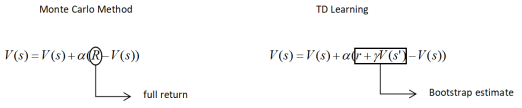
\includegraphics[scale=1.0]{pix/comparison_MC_and_TD.png}
\caption{A comparison between MC and TD learning}
%\label{fig:label}
\end{figure}
\noindent Thus, our temporal difference learning update rule is equation 
(\ref{learning_update_rule_TD}).

We learned that $r + \gamma V(s')$ is an estimate of the value of state $V(s)$. 
So, we can call $r + \gamma V(s')$ the TD target. Thus, subtracting $V(s)$ 
from $r + \gamma V(s')$ implies that we are subtracting the predicted value 
from the target value, and this is usually called the TD error. Okay, what 
about that $\alpha$? It is basically the learning rate, also called the step 
size. That is: 

$$
V(s) = V(s) + \underbrace{\alpha}_{\text{learning rate}}
(\underbrace{r + \gamma V(s') - V(s)}_{\text{TD error})
$$

Our TD learning update rule basically implies:  

Value of a state = value of a state + learning rate (reward + discount factor(value 
of next state) – value of a state)  


%+++++++++++++++++++++++++++++++++++++++++++
\subsection{Summary of Temporal Difference Learning}

In this section, we explored the TD learning update rule and how temporal 
difference learning is used to estimate the value of a state. Further study 
should explore the TD prediction algorithm so readers can get a clearer 
understanding of the TD learning method. Master classic RL, deep RL, 
distributional RL, inverse RL, and more with OpenAI Gym and TensorFlow. 


%+++++++++++++++++++++++++++++++++++++++++++
\subsection{Bellman Equation}

% https://www.geeksforgeeks.org/bellman-equation/

According to the Bellman Equation, long-term-reward in {\bf a given action is equal 
to the reward from the current action combined with the expected reward from the 
future actions} taken at the following time. Let's try to understand first.

\subsubsection{Exmaple}

Here we have a maze which is our environment and the sole goal of our agent is to 
reach the trophy state (R = 1) or to get Good reward and to avoid the fire state 
because it will be a failure (R = -1) or will get Bad reward.

\begin{figure}[H]
\centering
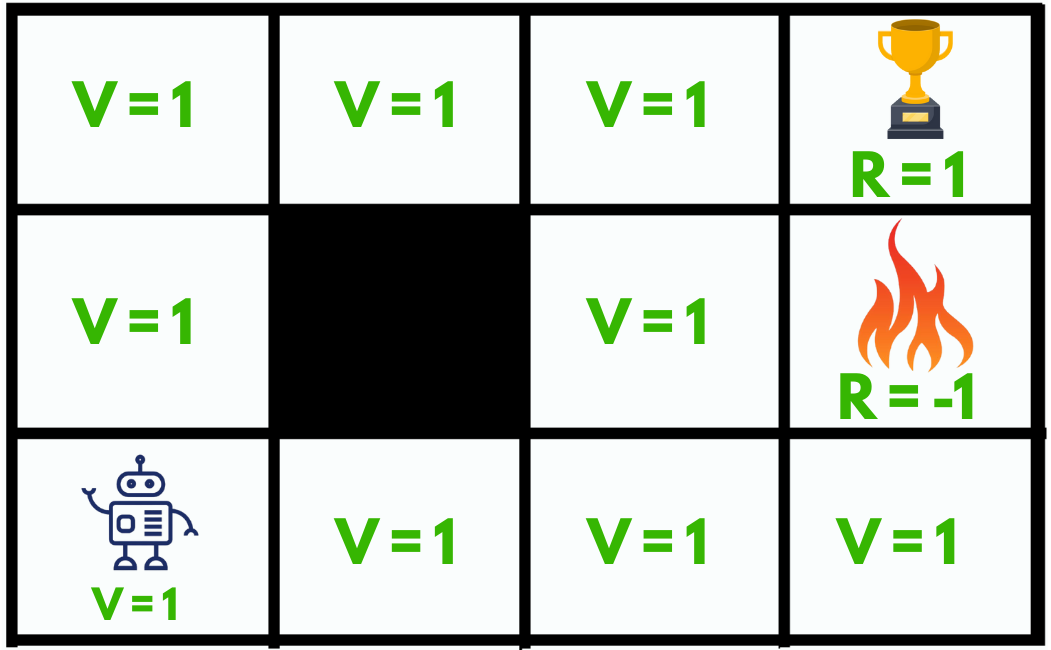
\includegraphics[scale=0.3]{pix/maze.png}
\caption{Without Bellman Equation}
%\label{fig:label}
\end{figure}

\subsubsection{What happens without Bellman Equation?}

Initially, we will give our agent some time to explore the environment and let it 
figure out a path to the goal. As soon as it reaches its goal, it will back trace 
its steps back to its starting position and mark values of all the states which 
eventually leads towards the goal as V = 1.

The agent will face no problem until we change its starting position, as it will 
not be able to find a path towards the trophy state since the value of all the 
states is equal to 1. 

\subsubsection{Bellman equation}

To solve the above problem we should use Bellman Equation:
$$
V(s) = max_a\left( R(s,a) + \gamma V(s') \right)
$$

State($s$): current state where the agent is in the environment

Next State($s'$): After taking action($a$) at state($s$) the agent reaches $s'$

Value($V$): Numerica representation of a state which helps the agent to find its
path. $V(s)$ here means the value of the state $s$.

Reward($R$): treat which the agent gets after performing an action($a$).

\begin{itemize}
%\setlength{\itemsep}{0pt}
%\setlength{\parsep}{0pt}
\setlength{\parskip}{0pt}
\item[-]
$R(s)$: reward for being in the state $s$

\item[-]
$R(s,a)$: reward for being in the state $s$ and performing an action $a$

\item[-]
$R(s,a,s')$: reward for being in a state $s$, taking an action $a$ and 
ending up in $s'$
\end{itemize}

e.g. Good reward can be $+1$, Bad reward can be $-1$, No reward can be $0$.

Action($a$): set of possible actions that can be taken by the agent in the 
state($s$). e.g. (LEFT, RIGHT, UP, DOWN)

Discount factor($\gamma$): determines how much the agent cares about rewards 
in the distant future relative to those in the immediate future. It has a value 
between $0$ and $1$. Lower value encourages short–term rewards while higher 
value promises long-term reward

\begin{figure}[H]
\centering
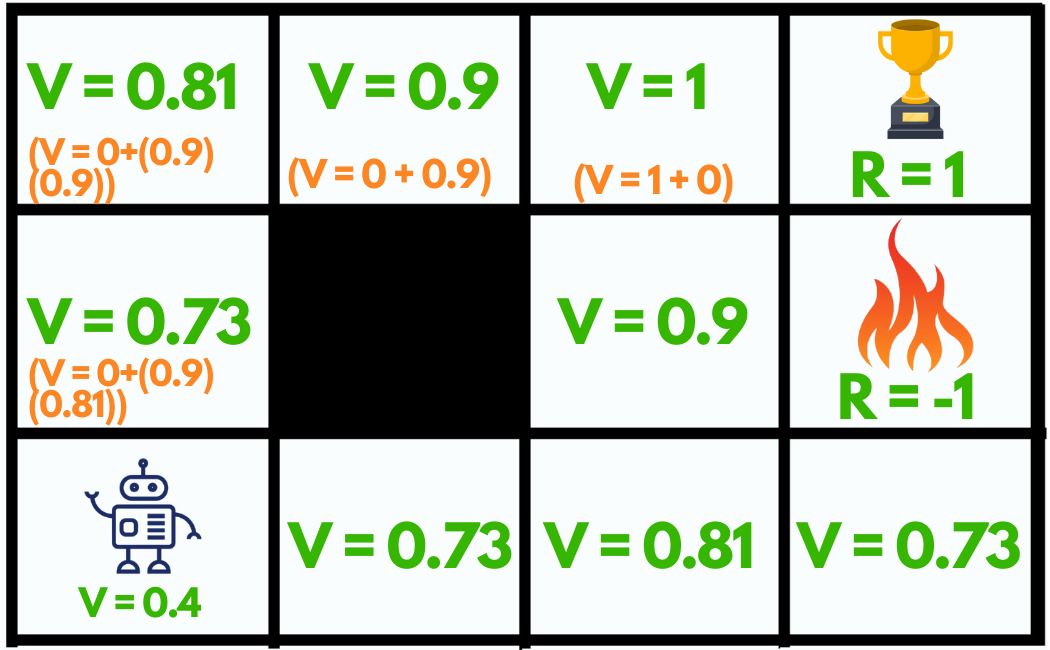
\includegraphics[scale=0.3]{pix/maze_bellman.png}
\caption{Using Bellman Equation}
%\label{fig:label}
\end{figure}

The max denotes the most optimum action among all the actions that the agent can 
take in a particular state which can lead to the reward after repeating this 
process every consecutive step.  

For example:

\begin{itemize}
%\setlength{\itemsep}{0pt}
%\setlength{\parsep}{0pt}
\setlength{\parskip}{0pt}
\item[-]
The state left to the fire state ($V = 0.9$) can go UP, DOWN, RIGHT but NOT LEFT 
because it's a wall(not accessible). Among all these actions available the maximum 
value for that state is the UP action.

\item[-]
The current starting state of our agent can choose any random action UP or RIGHT 
since both lead towards the reward with the same number of steps.
\end{itemize}

By using the Bellman equation our agent will calculate the value of every step 
except for the trophy and the fire state (V = 0), they cannot have values since 
they are the end of the maze.

So, after making such a plan our agent can easily accomplish its goal by just 
following the increasing values.


%+++++++++++++++++++++++++++++++++++++++++++
\subsection{one-step TD}
% https://trunghng.github.io/artificial-intelligent/reinforcement-learning/2022/04/08/td-learning.html



%+++++++++++++++++++++++++++++++++++++++++++
\subsection{n-step TD Prediction}
% http://www.incompleteideas.net/book/7/node2.html



